\section{Resultados Esperados}
Los entregables como resultado de este trabajo terminal serán los siguientes:
\begin{itemize}
    \item Una herramienta de software que permita la comunicación mediante alertas entre los usuarios y sus contactos de emergencia.
    \item Un sistema electrónico que permita la medición de los niveles de alcohol en la sangre de un individuo, así como la acción de bloqueo del “switch” de encendido del auto.
\end{itemize}
Se pretende que el prototipo final del sistema electrónico sea adaptable a un automóvil para poder permitir el bloqueo total al momento de encenderlo si no se cumple con la tasa de control de alcoholemia. En la Figura \ref{fig:prop_sol} se muestra la propuesta de solución.
\begin{center}
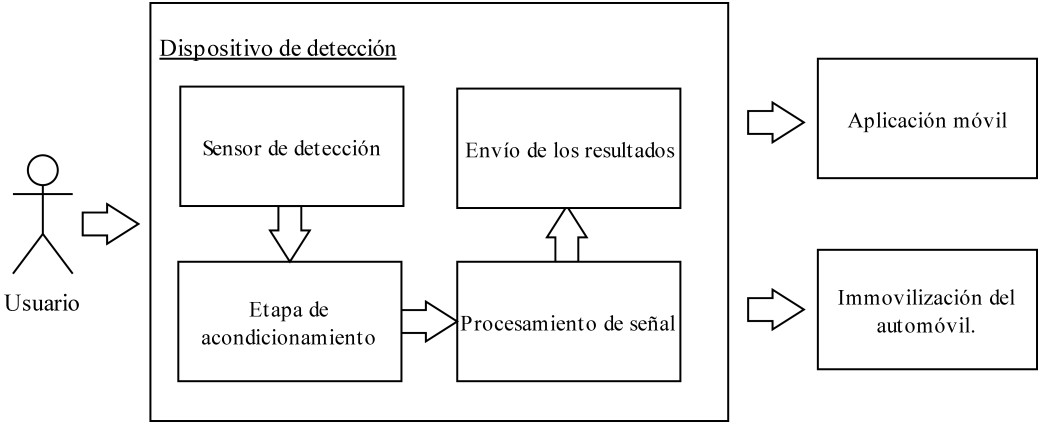
\includegraphics[scale=1]{Capitulo1/img/propuesta_de_solucion.jpg}
\captionof{figure}{Propuesta de Solución.}
\label{fig:prop_sol}
\end{center}